\documentclass[och, master]{SCWorks}

\usepackage[utf8]{inputenc}
\usepackage[T2A]{fontenc}
\usepackage[russian]{babel}

\usepackage{pdfpages}

\usepackage{hyperref}
\usepackage{amsfonts}
\usepackage{commath}
\usepackage{amsthm}

\theoremstyle{plain}
\newtheorem{thethm}{Теорема}

\theoremstyle{plain}
\newtheorem{lemma}{Лемма}

\theoremstyle{plain}
\newtheorem{note}{Замечание}

\theoremstyle{definition}
\newtheorem{defn}{Определение} 

\newtheorem{exmp}{Пример}

\geometry{verbose,a4paper,tmargin=2cm,bmargin=2cm,lmargin=2.5cm,rmargin=1.5cm}

\hypersetup{
    colorlinks=true, %set true if you want colored links
    linktoc=all,     %set to all if you want both sect. and subsect. linked
    linkcolor=blue,  %choose some color if you want links to stand out
}

\author{Sharov Alex}

\begin{document}

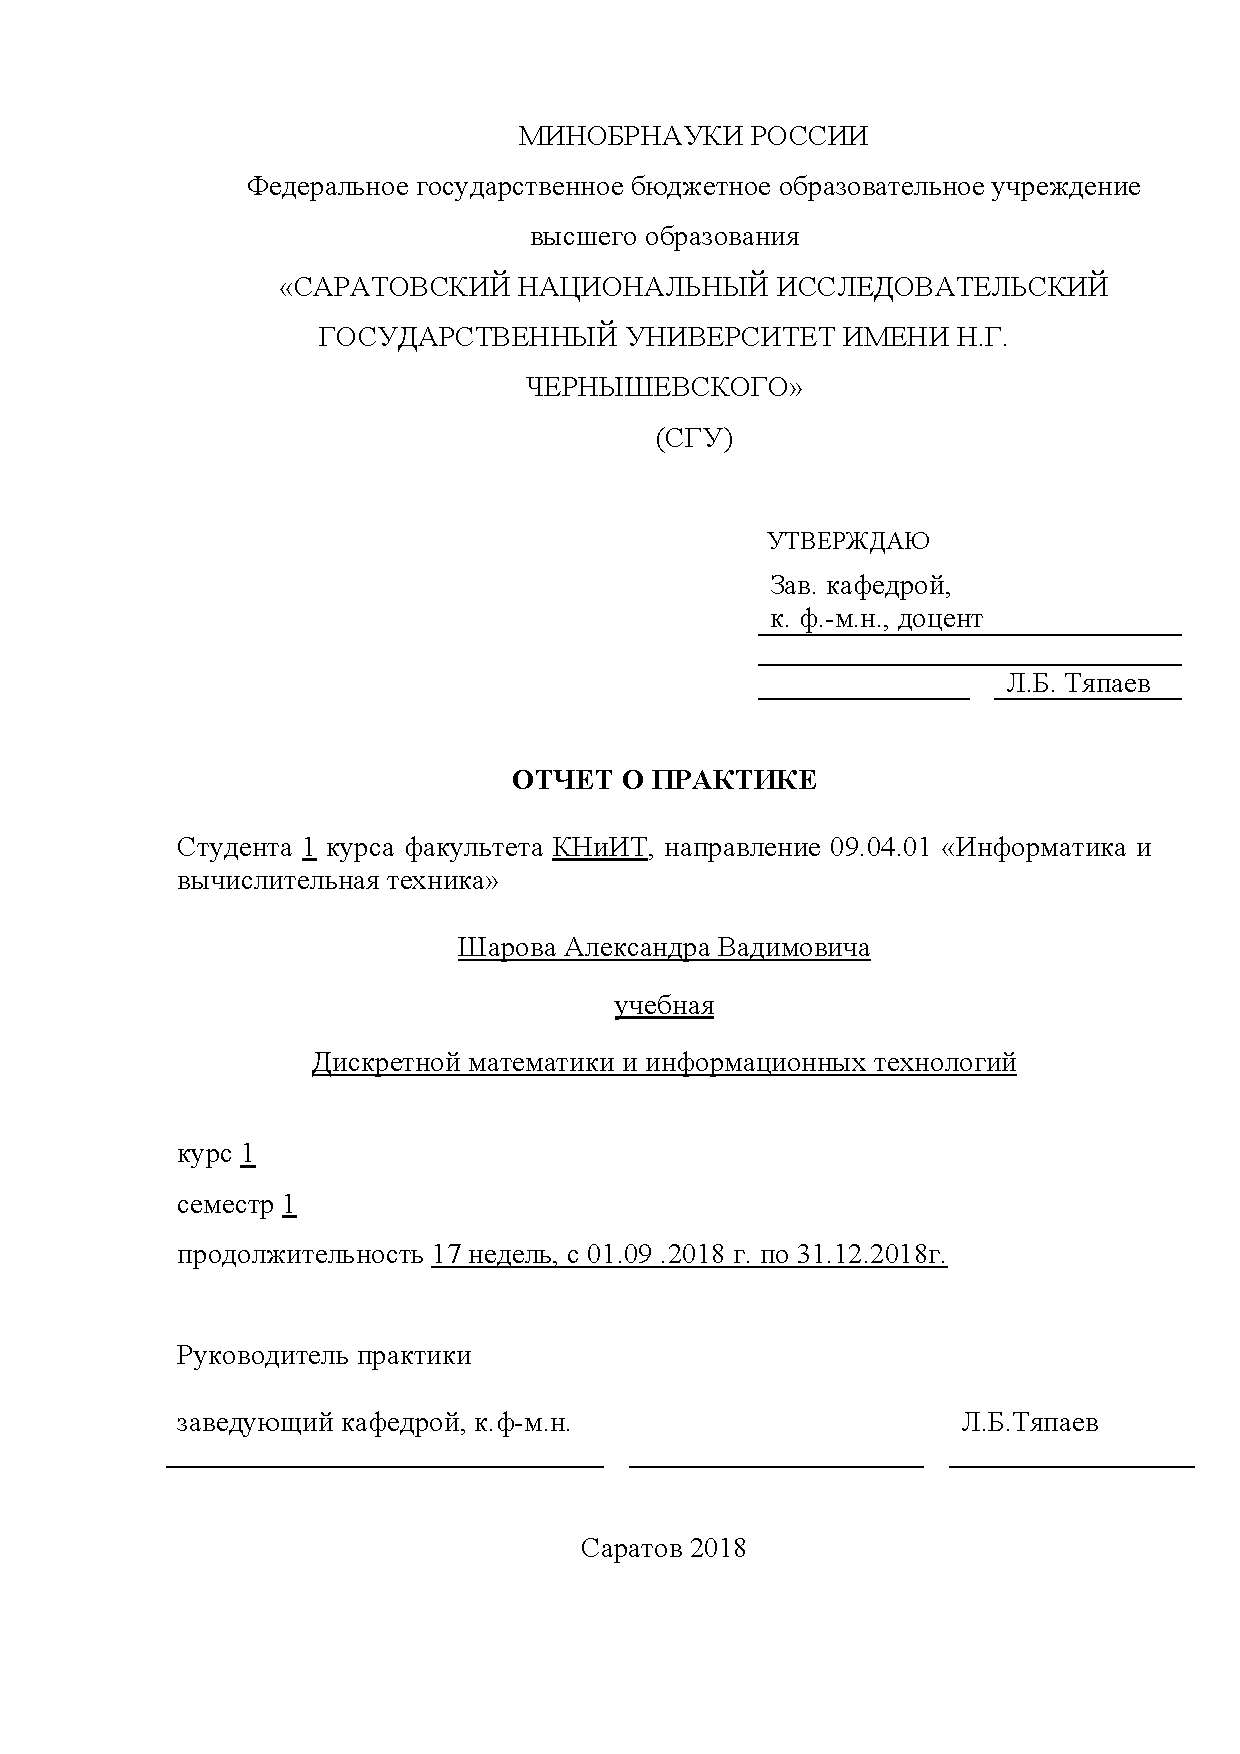
\includepdf[pages={1}]{titul.pdf}
\setcounter{tocdepth}{1}

\tableofcontents

\definitions

\begin{enumerate}
	\item $\mathbb {Z}$ -- кольцо целых рациональных чисел
	\item $\mathbb {Z}_{+}$ -- множество натуральных чисел $\mathbb {N}$
	\item ${N}_0=\{0,1,\dots\}$
	\item $\mathbb {P}$ -- множество простых чисел
	\item Сепарабельное пространство -- топологическое пространство, в котором можно выделить счётное всюду плотное подмножество
	\item Плотное множество -- подмножество пространства, точками которого можно сколь угодно хорошо приблизить любую точку объемлющего пространства.
	\item Счётное множество -- бесконечное множество, элементы которого возможно пронумеровать натуральными числами.
	\item Хаусдорфово пространство — топологическое пространство, удовлетворяющее сильной аксиоме отделимости $T_2$.
	\item Множество из $\mathbb {R}^n$ называется компактом, если из любой последовательности его точек можно выделить сходящуюся подпоследовательность, предел которой принадлежит этому множеству.
	\item Локально компактное пространство — топологическое пространство, у каждой точки которого существует открытая окрестность, замыкание которой компактно.
	\item Размерностью полного метрического пространства $X$ называется наименьшее целое число $n$ такое, что для любого покрытия пространства $X$ существуют вписанное в него подпокрытие кратности $n+1$.
\end{enumerate}

\intro
Со времен Ньютона и Лейбница вещественные числа применялись как основной математический объект, который казалось бы отлично подходил для описания окружающего мира. В большинстве практических задач обычно составлялись уравнения и в последствии искалось числовое решение над полем действительных чисел $\mathbb {R}$. Обоснования почему в качестве описательного элемента выбрали именно поле $\mathbb {R}$ даже не стоял. В качестве пространства стандартом де-факто долгое время являлось пространство $\mathbb {R}^3$, а уже после открытий Римана и Эйнштейна $\mathbb {R}^4$. 

С течением времени и наращиванием математического аппарата представление о том, что пространство $\mathbb {R}^3$ является наиболее подходящим для описания реального мира все усиливалось, но надо понимать, что евклидово пространство $\mathbb {R}^3$ не более чем удачно выбранная модель описания реального физического пространства. 

Так как реальный мир построен на евклидовой геометрии, то получается, что и она очень хорошо описывается вещественными числами, но в случае если бы мы могли отказаться от использования данной геометрии для изучения реального мира мы бы могли отказаться и от вещественной числовой системы. Но какую выбрать систему в данном случае? На этот ответ лучше всего отвечает теория $p$-адического исчисления, которая является с математической точки зрения более подходящей для описания тех объектов, с которыми приходиться работать в задачах физики, биологии и криптографии.\cite{bib:kozirev:2008}

Целью данной научной работы является изучение основ $p$-адического анализа на поле $\mathbb {Z}_p$. В данной работе будут рассмотрены такие понятия как $p$-адическое числа, пространства, функции и $p$-адическая дифференцируемость. В качестве наглядного примера отличия анализа на $\mathbb {R}$ и на $\mathbb {Z}_p$ будет рассмотрена теорема о среднем значении.

\section{p-Адические числа}

\subsection{p-Адическая норма}

\begin{defn}
Пусть $M$ - некоторое непустое множество, и пусть \linebreak ${d: M \times M \rightarrow \mathbb {R}_{\ge0}}$ -- функция двух переменных, определенная на этом множестве и принимающая значения во множестве действительных неотрицательных чисел. Функция $d$ называется метрикой (а множество $M$ -- метрическим пространством), если $d$ удоволетворяет трем условиям:

\begin{enumerate} 
	\item Для каждой пары $a, b \in M$ справедливо: $d(a, b)=0$ тогда и только тогда, когда $a=b$.
	\item Для каждой пары $a, b \in M$ справедливо равенство $d(a, b) = d(b, a)$.
	\item Для каждой тройки $a, b, c \in M$ справедливо неравенство $d(a, b) \le d(a, c) + d(c, b)$.
\end{enumerate}
\end{defn}

\begin{exmp}
Множество $\mathbb {R}$ всех действительных чисел есть метрическое пространство с метрикой $d(a, b)= \abs{a-b}$, где $\abs{.}$ есть абсолютная величина.
\end{exmp}


\begin{defn}
Функция $\norm{.}$, определенная на произвольном коммутативном кольце R и принимающая значения в $\mathbb {R}_{\ge 0}$ называется нормой (также, абсолютной величиной), если она удовлетворяет следующим условиям:

\begin{enumerate} 
	\item Для любого $a \in R$ справедливо, что $\norm{a}=0$ тогда и только тогда, когда $a=0$.
	\item Для каждой пары $a, b \in R$ справедливо равенство $\norm{a \cdot b} = \norm{a} \cdot \norm{b}$.
	\item Для каждой пары $a, b \in R$ справедливо неравенство треугольника: $\norm{a + b} \le \norm{a} + \norm{b}$
\end{enumerate}
\end{defn}

Из определения следует, что если положить $d(a, b)= \norm{a - b}$, то фактически будет задана метрика $d$ на кольце $R$. Данная метрика называется метрикой, индуцированной нормой $\norm{.}$.

\begin{defn}
Пусть $p \in \mathbb {P}$ -- некоторое простое число. В поле $\mathbb {Q}$ введем другую норму $\norm{.}_p$ по правилу:

\begin{enumerate} 
	\item $\norm{0}_p = 0$,
	\item $\norm{n}_p = p ^ {-ord_pn}$,
\end{enumerate}

\noindent где $n > 0$ некоторое натуральное число, а $ord_pn$ показатель степени, в которой число $p$ входит в это произведение. В этом случае норма $\norm{.}_p$ называется $p$-адической нормой.
\end{defn}

Норма $\norm{.}_p$  удовлетворяет всеми характерными свойствами нормы даже в более сильной форме, а именно:

\begin{enumerate} 
	\item $\norm{x}_p \ge 0$, причем $\norm{x}_p = 0$ если $x = 0$.
	\item $\norm{xy}_p = \norm{x}_p \cdot \norm{y}_p$.
	\item $\norm{x + y}_p \le \max(\norm{x}_p, \norm{y}_p)$ \cite{bib:analysis:volovich}
\end{enumerate}

Заметим, что норма $\norm{x}_p$ может принимать лишь счетное число значений $p ^ {-ord_pn}$.

Также, норма $\norm{x}_p$ определяет ультраметрику на $\mathbb {Q}$. Данная норма неархимедова, так как $\norm{nx}_p \le \norm{x}_p \forall n \in \mathbb {Q}_{+}$.

\begin{thethm}
	Нормы $\norm{.}$ и $\norm{.}_p$ $\forall p = 2, 3, \dots$ исчерпывают все нетривиальные неэквивалентные нормы поля рациональных чисел $\mathbb {Q}$.
\end{thethm}


\subsection{p-Адические числа}

\begin{defn}
Пополнение поля $\mathbb {Q}$ по $p$-адической норме образует поле $\mathbb {Q}_p$ $p$-адических чисел. Поле $\mathbb {Q}_p$ аналогично полю $\mathbb {R} = \mathbb {Q}_{\infty}$ вещественных чисел, получаемых пополнение поля $\mathbb {Q}$ по норме $\norm{x}=\norm{x}_{\infty}$.
\end{defn}


\begin{defn}
Любое $p$-адическое число $x \ne 0$ однозначно представляется в каноническом виде

\begin{equation} \label{numbers:decomposition}
	x = p^{\gamma} \cdot (x_0 + x_1\cdot p + x_2 \cdot p^2 + \dots
\end{equation}

\noindent где $\gamma = \gamma(x) \in \mathbb {Z}$ и $x_j$ -- целые числа такие, что $0 \le x_j \le p-1$, $x_0 > 0,$ \linebreak $(j=0,1,\dots)$. 
\end{defn}

Представление \eqref{numbers:decomposition} аналогично разложению любого вещественного числа $x$ в бесконечную десятичную дробь:
\begin{equation*}
\begin{aligned}
	x=\pm10^\gamma \cdot (x_0 + x_1 \cdot 10^{-1} + x_2 \cdot 10^{-2} + \dots),\\
	\gamma \in \mathbb {Z}, x_j = 0, 1, \dots, 9, x_0 > 0,
\end{aligned}
\end{equation*}

\noindent и доказывается аналогично.

Помимо разложения, представление \eqref{numbers:decomposition} дает рациональные числа тогда и только тогда, когда, начиная с некоторого номера числа $x_j, j=0,1,\dots$ образуют периодическую последовательность.

\begin{defn}
Поле $\mathbb {Q}_p$ является коммутативно-ассоциативной группой по сложению;
\end{defn}

\begin{defn}
Поле $\mathbb {Q}_p^*=\mathbb {Q}_p \setminus \{0\}$ является коммутативно-ассоциативной группой по умножению;
\end{defn}

\begin{defn}
Поле $\mathbb {Q}_p^*$ называется мультипликативной группой поля $\mathbb {Q}_p$\cite{bib:analysis:baker};
\end{defn}

\begin{defn}
$p$-адические числа $x$, для которых $\norm{x}_p \le 1$ (т.e. $\gamma(x) \ge 0$ или $\{x\}_p=0$), называются целыми $p$-адическими числами, и их множество обозначается $\mathbb {Z}_p$. Множество $\mathbb {Z}_p$ является подкольцом кольца $\mathbb {Q}_p$; $\mathbb {Z}_+$ плотно в $\mathbb {Z}_p$. Целые числа $x \in \mathbb {Z}_p$, для которых $\norm{x}_p=1$, называютсяются единицами в $\mathbb {Z}_p$. \cite{bib:analysis:vladimirov}
\end{defn}

Совокупность элементов $x$ из $\mathbb {Z}_p$, для которых $\norm{x}_p < 1$ (т.e. $\gamma(x) \ge 0$ или $\norm{x}_p \le \frac{1}{p}$) образуют главный идеал кольца $\mathbb {Z}_p$; Данный идеал имеет вид $p\mathbb {Z}_p$. Поле вычетов $\mathbb {Z}_p \setminus p\mathbb {Z}_p$ состоит из $p$ элементов. В мультипликативной группе поля $\mathbb {Z}_p \setminus p\mathbb {Z}_p$ существует единица $\eta \ne 1$ порядка $p-1$ такая, что элементы $0, \eta, \eta^2, \dots, \eta^{p-1} = 1$ образуют полный набор представителей классов вычетов поля $\mathbb {Z}_p \setminus p\mathbb {Z}_p$.

\subsection{Пространство p-адических чисел $\mathbb {Q}_p$}
В силу свойств $p$-адической нормы норма в поле $\mathbb {Q}_p$ удовлетворяет неравенству треугольника:
$$\norm{x + y}_p \le \max(\norm{x}_p, \norm{y}_p) \le \norm{x}_p + \norm{y}_p, x,y \in \mathbb {Q}_p.$$
\noindent Следовательно в $\mathbb {Q}_p$ можно ввести метрику:

\begin{equation}
	\rho (x,y)=\norm{x-y}_p.
\end{equation}

\noindent При этом $\mathbb {Q}_p$ становится полным метрическим пространством. Из представления \eqref{numbers:decomposition} следует сепарабельность $\mathbb {Q}_p$.  

\begin{defn}
$B_{\gamma}(a)$ -- круг радиуса $p^{\gamma^p}$ с центром в точке $a \in \mathbb {Q}_p$:
\begin{equation}
	B_\gamma(a) = \bigg\{x: \norm{x-a}_p \le p^{\gamma} \bigg\}, \gamma \in \mathbb {Z}
\end{equation}
\end{defn}

\begin{defn}
$S_{\gamma}(a)$ -- граница радиуса $p^{\gamma^p}$.
\begin{equation}
	S_\gamma(a) = \bigg\{x: \norm{x-a}_p = p^{\gamma} \bigg\}, \gamma \in \mathbb {Z}
\end{equation}
\end{defn}

\begin{lemma}
Если $b \in B_{\gamma}(a)$, то $B_{\gamma}(b)=B_{\gamma}(a)$.
\end{lemma}

\begin{note}
Круг $B_{\gamma}(a)$ и окружность $S_{\gamma}(a)$ -- открыто-замкнутые множества в $\mathbb {Q}_p$.
\end{note}

\begin{note}
Всякая точка круга $B_{\gamma}(a)$ является его центром.
\end{note}

\begin{note}
Любые два круга в $\mathbb {Q}_p$ либо не имеют общих точек, либо один содержится в другом.
\end{note}

\begin{note}
Всякое открытое множество в $\mathbb {Q}_p$ есть объединение не более чем счетного числа кругов без общих точек.
\end{note}

\begin{lemma} \label{lemma:2}
Если множество $M \subset \mathbb {Q}_p$ содержит две различные точки $a$ и $b$, $a \ne b$, то его можно представить в виде объединения непересекающихся открыто-замкнутых (в $M$) множеств $M_1, M_2$ таких, что $a \in M_1, b \in M_2$.
\end{lemma}

Лемма \eqref{lemma:2} утверждает, что всякое множество пространства $\mathbb {Q}_p$, состоящее из более чем одной точки, несвязно. Другими словами, связная компонента любой точки совпадает с самой точкой. Из этого следует, что $\mathbb {Q}_p$ является вполне несвязным пространством.

Если рассматривать лемму для случая, когда множество $M$ состоит только из двух точек $a$ и $b$, убеждаемся, что существует непересекающиеся окрестности этих точек. Из этого можно сделать вывод, что пространство $\mathbb {Q}_p$ хаусдорфово.

\begin{lemma}
Для того чтобы множество $K \subset \mathbb {Q}_p$ было компактом, необходимо и достаточно, чтобы оно было замкнутым и ограниченным в $\mathbb {Q}_p$
\end{lemma}

\begin{note}
Всякий круг $B_{\gamma}(a)$ является и окружность $S_{\gamma}(a)$ компакты.
\end{note}

\begin{note}
Пространство $\mathbb {Q}_p$ локально компактное.
\end{note}

\begin{note}
Всякий компакт можно покрыть конечным числом кругов фиксированного радиуса без общих точек.
\end{note}

\begin{note}
В пространстве $\mathbb {Q}_p$ справедлива лемма Гейне-Бореля: из каждого бесконечного покрытия компакта $K$ можно выбрать конечное покрытие $K$.
\end{note}

\begin{thethm}
Размерность пространства $\mathbb {Q}_p$ равна $0$.
\end{thethm}

\section{p-Адический анализ в $\mathbb {Z}_p$}

Так как компакт $\mathbb {Z}_p$ есть пополнение множества $\mathbb {N}_0$ по метрике \linebreak ${d_p(x,y)=\norm{x-y}_p}$, то любое число из $\mathbb {Z}_p$ есть предел последовательности чисел из $\mathbb {N}_0$.

\begin{defn}
$p$-адическое целое $z$ является пределом последовательности $\{z_i\}^{\infty}_{i=0}$, если если для любого $\epsilon > 0$ найдется $N$ такое, что $\norm{z_i-z}_p < \epsilon$ как только $i>N$. \cite{bib:analysis:anashin}
\end{defn}

\begin{defn}
$p$-адическое целое $z$ есть предел последовательности $\{z_i\}^{\infty}_{i=0}$, если для любого (достаточно большого) положительного рационального целого $K$ найдется $N$ такое, что ${z_i \equiv z \pmod p^K}$ при всех $i>N$. \cite{bib:analysis:anashin}
\end{defn}

\begin{note}
По определению $p$-адической метрики $\norm{z_i-z}_p \le p^{-K}$ тогда и только тогда, когда $z_i \equiv z \pmod p^K$. \cite{bib:analysis:anashin}
\end{note}

\begin{defn}
Функция $f:\mathbb {Z}_p \rightarrow \mathbb {Z}_p$ называется непрерывной в точке $z \in \mathbb {Z}_p$, если для любого (достаточно большого) положительного рационального целого $M$ найдется положительное рациональное целое $L$ такое, что ${f(x) \equiv f(z) \pmod p^M}$ как только $x \equiv z \pmod{p^L}$. \cite{bib:analysis:anashin}
\end{defn}

\begin{defn}
Функция $f$ называется равномерно непрерывной на $\mathbb {Z}_p$, если $f$ непрерывна в каждой точке $z \in \mathbb {Z}_p$, и $L$ зависит только от $M$ и не зависит от $z$.\cite{bib:analysis:ciocan}
\end{defn}


\subsection{$p$-адическая дифференцируемость}

\begin{defn}
Функция $f:\mathbb {Z}_p \rightarrow \mathbb {Z}_p$ называется дифференцируемой в точке $z \in \mathbb {Z}_p$, если существует $p$-адическое число $f'(x) \in \mathbb {Q}_p$ такое, что для любого $M \in \mathbb {N}$ справедливо
\begin{equation} \label{derivative:1}
	\norm{\frac{f(x+h)-f(x)}{h} - f'(x)}_p \le \frac{1}{p^M},
\end{equation}

\noindent если $h$ достаточно мало, т.e. когда $\norm{h}_p \le p^{-K}$, где $K=K(M)$ достаточно велико.
\end{defn}

\begin{defn}
Функция $f$ называется равномерно дифференцируемой (на $\mathbb {Z}_p$), если неравенство \eqref{derivative:1} выполняется одновременно для всех $x \in \mathbb {Z}_p$ как только $h$ достаточно мало. \cite{bib:analysis:anashin:en}
\end{defn}

\begin{lemma}
Если совместимая функция $f:\mathbb {Z}_p \rightarrow \mathbb {Z}_p$ дифференцируема в точке $x \in \mathbb {Z}_p$, то $f'(x) \in \mathbb {Z}_p$.
\end{lemma}

\begin{defn}
Функция $f:\mathbb {Z}_p \rightarrow \mathbb {Z}_p$ называется дифференцируемой в точке $x \in \mathbb {Z}_p$, если существует $p$-адическое число $f'(x) \in \mathbb {Q}_p$ такое, что для любого $M \in \mathbb {N}$ справедливо
\begin{equation} \label{derivative:2}
	f(x+h) \equiv f(x) + h \cdot f'(x) \pmod p^{M + ord_p h}
\end{equation}
\end{defn}

\begin{defn}
Функция $f$ называется равномерно дифференцируемой (на $\mathbb {Z}_p$), если неравенство \eqref{derivative:2} выполняется одновременно для всех $x \in \mathbb {Z}_p$ как только $h$ достаточно мало, т.e. когда $ord_p h \ge K=K(M)$ для достаточно большого $K \in \mathbb {N}$.
\end{defn}

\begin{note}
Правила дифференцирования не зависят от метрики: для вычисления производных суммы, частного и сложной функции в $p$-адическом анализе используются те же формулы, что и в действительном.
\end{note}

\begin{note}
Между действительным и $p$-адическим анализом существует резкое различие например в том, что в и в том, и в в другом случае производная константы равна $0$, однако в $p$-адическом анализе в отличии от действительного равенство нулю производной некоторой функции не означает, что эта функция константа.
\end{note}

\subsection{теорема о среднем}

\begin{thethm} (в $\mathbb {R}$)
Если функция $f(x)$ непрерывна на отрезке $[a, b]$ и дифференцируема на интервале $(a, b)$, то в этом интервале найдется хотя бы одна точка $\xi$, такая, что $f(b)-f(a)=f'(\xi)(b-a)$.
\end{thethm}

Ключевая проблема в доказательстве данной теоремы на поле $\mathbb {Q}_p$ в том, что поле $\mathbb {Q}_p$ неупорядоченное. Но эта трудность может быть устранена\cite{bib:analysis:gouvea}. В $\mathbb {R}$ мы можем переопределить среднее так, что:

$$ \xi=at+b(1-t) \quad \forall 0 \le t \le 1; $$

\noindent такое преобразование, к примеру, делается когда данная теорема доказывается в поле $\mathbb {C}$. Теперь мы можем написать $p$-адический аналог теоремы о среднем. 


\begin{thethm} (в $\mathbb {Q}_p$)\cite{bib:analysis:alain}
Если функция $f(x)$ дифференцируема и производная непрерывна на $\mathbb {Q}_p$, то для любых двух чисел $a$ и $b$ из множества $\mathbb {Q}_p$ найдется такой элемент $\xi \in \mathbb {Q}_p$, что:

$$ \xi=at+b(1-t) \quad \forall t: |t| \le 1$$

\noindent для которого:

$$ f(b)-f(a)=f'(\xi)(b-a).$$
\end{thethm}

\begin{proof}
Возьмем $f(x)=x^p-x, a=0, b=1$, тогда производная $f'(x)=px^{p-1}-1$ и $f(a)=f(b)=0$. Теорема предполагает, что существует такое число $\xi: {p\xi^{p-1}-1=0}$. В свою очередь любое $\xi=at+b(1-t)=(1-t)$, где $t \in \mathbb {Z}_p$ (это значит, что $t| \le 1$), должно принадлежать $\mathbb {Z}_p$. В свою очередь $p\xi^{p-1}-1$ принадлежит $\mathbb {Z}_p$ (а это принадлежит $1+p\mathbb {Z}_p$) и из-за этого не может быть нулем.
\end{proof}













\bibliographystyle{biblio/ugost}
\bibliography{biblio/biblio}

\end{document}